\documentclass[usenames,dvipsnames,tikz]{standalone}
\usepackage{xcolor}
\colorlet{tBlue}{RoyalBlue!35!Cerulean}
\colorlet{tRed}{Red}
\usepackage{tikz}
\usepackage{standalone}
\begin{document}
	
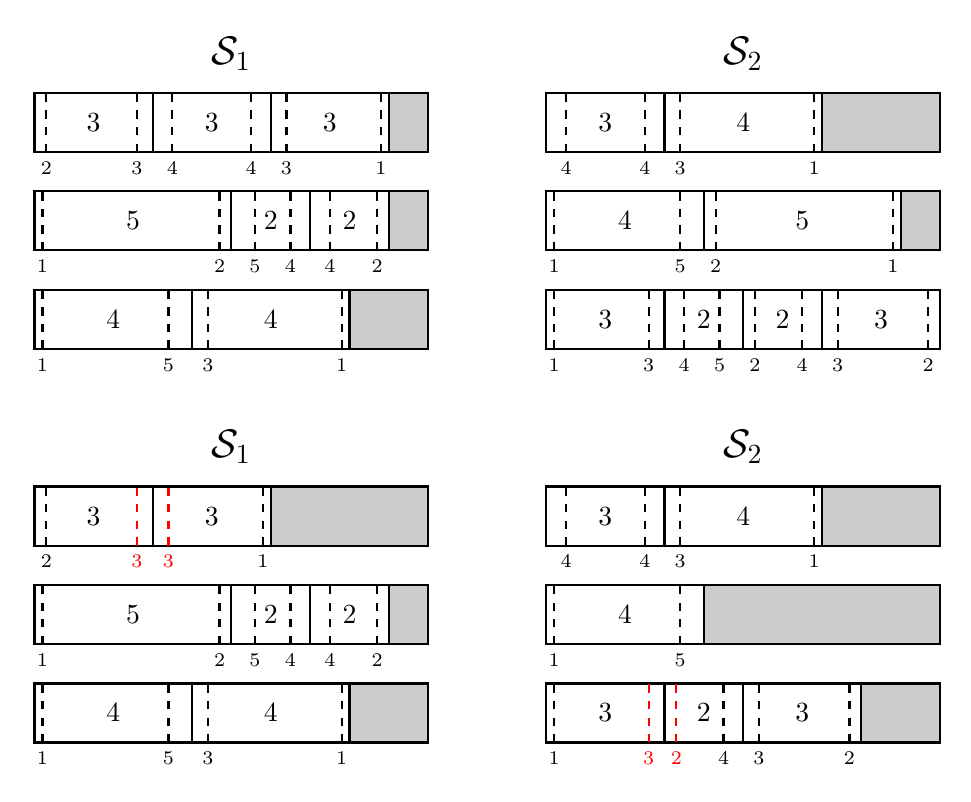
\begin{tikzpicture}
%\draw [help lines] (-1,-2) grid (17,10);
% 1=0.1, 2=0.15, 3=0.2, 4=0.25, 5=0.3

%Parent 1
\node at (2.5, 8.75) {\Large{$\mathcal{S}_1$}};
\draw [thick] (0,5) rectangle (5,5.75);
\draw [thick] (0,6.25) rectangle (5,7);
\draw [thick] (0,7.5) rectangle (5,8.25);

%bottom row, 4, 4 (1-5, 3-1)
\draw [thick] (2,5) -- (2,5.75);
\draw [thick] (4,5) -- (4,5.75);
\filldraw[fill=black!20!white, draw=black, thick] (4,5) rectangle (5,5.75);
\draw [thick, dashed] (0.1,5) -- (0.1,5.75);
\draw [thick, dashed] (1.7,5) -- (1.7,5.75);
\draw [thick, dashed] (2.2,5) -- (2.2,5.75);
\draw [thick, dashed] (3.9,5) -- (3.9,5.75);
\node [below] at (0.1,5) {\scriptsize{1}};
\node [below] at (1.7,5) {\scriptsize{5}};
\node [below] at (2.2,5) {\scriptsize{3}};
\node [below] at (3.9,5) {\scriptsize{1}};
\node at (1,5.375) {4};
\node at (3,5.375) {4};
%\node at (1,5.15) {\footnotesize{4}};
%\node at (1,5.5) {G};
%\node at (3,5.15) {\footnotesize{4}};
%\node at (3,5.5) {F};


%middle row, 5, 2, 2 (1-2, 5-4, 4-2)
\draw [thick] (2.5,6.25) -- (2.5,7);
\draw [thick] (3.5,6.25) -- (3.5,7);
\filldraw[fill=black!20!white, draw=black, thick] (4.5,6.25) rectangle (5,7);
\draw [thick, dashed] (0.1,6.25) -- (0.1,7);
\draw [thick, dashed] (2.35,6.25) -- (2.35,7);
\draw [thick, dashed] (2.8,6.25) -- (2.8,7);
\draw [thick, dashed] (3.25,6.25) -- (3.25,7);
\draw [thick, dashed] (3.75,6.25) -- (3.75,7);
\draw [thick, dashed] (4.35,6.25) -- (4.35,7);
\node [below] at (0.1,6.25) {\scriptsize{1}};
\node [below] at (2.35,6.25) {\scriptsize{2}};
\node [below] at (2.8,6.25) {\scriptsize{5}};
\node [below] at (3.25,6.25) {\scriptsize{4}};
\node [below] at (3.75,6.25) {\scriptsize{4}};
\node [below] at (4.35,6.25) {\scriptsize{2}};
\node at (1.25,6.625) {5};
\node at (3,6.625) {2};
\node at (4,6.625) {2};
%\node at (1.25,6.4) {\footnotesize{5}};
%\node at (1.25,6.75) {H};
%\node at (3,6.4) {\footnotesize{2}};
%\node at (3,6.75) {B};
%\node at (4,6.4) {\footnotesize{2}};
%\node at (4,6.75) {A};


%top row, 3, 3, 3 (2-3, 4-4, 3-1)
\draw [thick] (1.5,7.5) -- (1.5,8.25);
\draw [thick] (3,7.5) -- (3,8.25);
\draw [thick] (4.5,7.5) -- (4.5,8.25);
\filldraw[fill=black!20!white, draw=black, thick] (4.5,7.5) rectangle (5,8.25);
\draw [thick, dashed] (0.15,7.5) -- (0.15,8.25);
\draw [thick, dashed] (1.3,7.5) -- (1.3,8.25);
\draw [thick, dashed] (1.75,7.5) -- (1.75,8.25);
\draw [thick, dashed] (2.75,7.5) -- (2.75,8.25);
\draw [thick, dashed] (3.2,7.5) -- (3.2,8.25);
\draw [thick, dashed] (4.4,7.5) -- (4.4,8.25);
\node [below] at (0.15,7.5) {\scriptsize{2}};
\node [below] at (1.3,7.5) {\scriptsize{3}};
\node [below] at (1.75,7.5) {\scriptsize{4}};
\node [below] at (2.75,7.5) {\scriptsize{4}};
\node [below] at (3.2,7.5) {\scriptsize{3}};
\node [below] at (4.4,7.5) {\scriptsize{1}};
\node at (0.75,7.875) {3};
\node at (2.25,7.875) {3};
\node at (3.75,7.875) {3};

%-----------------------------------------------------------

%Parent 2
\node at (9,8.75) {\Large{$\mathcal{S}_2$}};
\draw [thick] (6.5,5) rectangle (11.5,5.75);
\draw [thick] (6.5,6.25) rectangle (11.5,7);
\draw [thick] (6.5,7.5) rectangle (11.5,8.25);

%bottom row, 3, 2, 2, 3 (1-3, 4-5, 2-4, 3-2)
\draw [thick] (8,5) -- (8,5.75);
\draw [thick] (9,5) -- (9,5.75);
\draw [thick] (10,5) -- (10,5.75);
\draw [thick, dashed] (6.6,5) -- (6.6,5.75);
\draw [thick, dashed] (7.8,5) -- (7.8,5.75);
\draw [thick, dashed] (8.25,5) -- (8.25,5.75);
\draw [thick, dashed] (8.7,5) -- (8.7,5.75);
\draw [thick, dashed] (9.15,5) -- (9.15,5.75);
\draw [thick, dashed] (9.75,5) -- (9.75,5.75);
\draw [thick, dashed] (10.2,5) -- (10.2,5.75);
\draw [thick, dashed] (11.35,5) -- (11.35,5.75);
\node [below] at (6.6,5) {\scriptsize{1}};
\node [below] at (7.8,5) {\scriptsize{3}};
\node [below] at (8.25,5) {\scriptsize{4}};
\node [below] at (8.7,5) {\scriptsize{5}};
\node [below] at (9.15,5) {\scriptsize{2}};
\node [below] at (9.75,5) {\scriptsize{4}};
\node [below] at (10.2,5) {\scriptsize{3}};
\node [below] at (11.35,5) {\scriptsize{2}};
\node at (7.25,5.375) {3};
\node at (8.5,5.375) {2};
\node at (9.5,5.375) {2};
\node at (10.75,5.375) {3};

%middle row, 4, 5 (1-5, 2-1)
\draw [thick] (8.5,6.25) -- (8.5,7);
\draw [thick] (11,6.25) -- (11,7);
\filldraw[fill=black!20!white, draw=black, thick] (11,6.25) rectangle (11.5,7);
\draw [thick, dashed] (6.6,6.25) -- (6.6,7);
\draw [thick, dashed] (8.2,6.25) -- (8.2,7);
\draw [thick, dashed] (8.65,6.25) -- (8.65,7);
\draw [thick, dashed] (10.9,6.25) -- (10.9,7);
\node [below] at (6.6,6.25) {\scriptsize{1}};
\node [below] at (8.2,6.25) {\scriptsize{5}};
\node [below] at (8.65,6.25) {\scriptsize{2}};
\node [below] at (10.9,6.25) {\scriptsize{1}};
\node at (7.5,6.625) {4};
\node at (9.75,6.625) {5};

%top row, 3, 4 (4-4, 3-1)
\draw [thick] (8,7.5) -- (8,8.25);
\draw [thick] (10,7.5) -- (10,8.25);
\filldraw[fill=black!20!white, draw=black, thick] (10,7.5) rectangle (11.5,8.25);
\draw [thick, dashed] (6.75,7.5) -- (6.75,8.25);
\draw [thick, dashed] (7.75,7.5) -- (7.75,8.25);
\draw [thick, dashed] (8.2,7.5) -- (8.2,8.25);
\draw [thick, dashed] (9.9,7.5) -- (9.9,8.25);
\node [below] at (6.75,7.5) {\scriptsize{4}};
\node [below] at (7.75,7.5) {\scriptsize{4}};
\node [below] at (8.2,7.5) {\scriptsize{3}};
\node [below] at (9.9,7.5) {\scriptsize{1}};
\node at (7.25,7.875) {3};
\node at (9,7.875) {4};


%AFTER ITEMS REMOVED %%%%%%%%%%%%%%%%%%%%%%%%%%%%%%%%%%%%%%%%%%%%%%%%%%%%%%%


%Parent 1
\node at (2.5, 3.75) {\Large{$\mathcal{S}_1$}};
\draw [thick] (0,0) rectangle (5,0.75);
\draw [thick] (0,1.25) rectangle (5,2);
\draw [thick] (0,2.5) rectangle (5,3.25);

%bottom row, 4, 4 (1-5, 3-1)
\draw [thick] (2,0) -- (2,0.75);
\draw [thick] (4,0) -- (4,0.75);
\filldraw[fill=black!20!white, draw=black, thick] (4,0) rectangle (5,0.75);
\draw [thick, dashed] (0.1,0) -- (0.1,0.75);
\draw [thick, dashed] (1.7,0) -- (1.7,0.75);
\draw [thick, dashed] (2.2,0) -- (2.2,0.75);
\draw [thick, dashed] (3.9,0) -- (3.9,0.75);
\node [below] at (0.1,0) {\scriptsize{1}};
\node [below] at (1.7,0) {\scriptsize{5}};
\node [below] at (2.2,0) {\scriptsize{3}};
\node [below] at (3.9,0) {\scriptsize{1}};
\node at (1,0.375) {4};
\node at (3,0.375) {4};

%middle row, 5, 2, 2 (1-2, 5-4, 4-2)
\draw [thick] (2.5,1.25) -- (2.5,2);
\draw [thick] (3.5,1.25) -- (3.5,2);
\filldraw[fill=black!20!white, draw=black, thick] (4.5,1.25) rectangle (5,2);
\draw [thick, dashed] (0.1,1.25) -- (0.1,2);
\draw [thick, dashed] (2.35,1.25) -- (2.35,2);
\draw [thick, dashed] (2.8,1.25) -- (2.8,2);
\draw [thick, dashed] (3.25,1.25) -- (3.25,2);
\draw [thick, dashed] (3.75,1.25) -- (3.75,2);
\draw [thick, dashed] (4.35,1.25) -- (4.35,2);
\node [below] at (0.1,1.25) {\scriptsize{1}};
\node [below] at (2.35,1.25) {\scriptsize{2}};
\node [below] at (2.8,1.25) {\scriptsize{5}};
\node [below] at (3.25,1.25) {\scriptsize{4}};
\node [below] at (3.75,1.25) {\scriptsize{4}};
\node [below] at (4.35,1.25) {\scriptsize{2}};
\node at (1.25,1.625) {5};
\node at (3,1.625) {2};
\node at (4,1.625) {2};

%CHANGED - top row, 3, 3 (2-3 X 3-1) (removed middle item, vsc violated)
\draw [thick] (1.5,2.5) -- (1.5,3.25);
\draw [thick] (3,2.5) -- (3,3.25);
\filldraw[fill=black!20!white, draw=black, thick] (3,2.5) rectangle (5,3.25);
\draw [thick, dashed] (0.15,2.5) -- (0.15,3.25);
\draw [thick, dashed, tRed] (1.3,2.5) -- (1.3,3.25);
\draw [thick, dashed, tRed] (1.7,2.5) -- (1.7,3.25);
\draw [thick, dashed] (2.9,2.5) -- (2.9,3.25);
\node [below] at (0.15,2.5) {\scriptsize{2}};
\node [below] at (1.3,2.5) {\textcolor{tRed}{\scriptsize{3}}};
\node [below] at (1.7,2.5) {\textcolor{tRed}{\scriptsize{3}}};
\node [below] at (2.9,2.5) {\scriptsize{1}};
\node at (0.75,2.875) {3};
\node at (2.25,2.875) {3};

%---------------------------------------------

%Parent 2
\node at (9,3.75) {\Large{$\mathcal{S}_2$}};
\draw [thick] (6.5,0) rectangle (11.5,0.75);
\draw [thick] (6.5,1.25) rectangle (11.5,2);
\draw [thick] (6.5,2.5) rectangle (11.5,3.25);

%CHANGED - bottom row, 3, 2, 3 (1-3 X 2-4, 3-2) (removed second item, vsc violated)
\draw [thick] (8,0) -- (8,0.75);
\draw [thick] (9,0) -- (9,0.75);
\draw [thick] (10.5,0) -- (10.5,0.75);
\filldraw[fill=black!20!white, draw=black, thick] (10.5,0) rectangle (11.5,0.75);
\draw [thick, dashed] (6.6,0) -- (6.6,0.75);
\draw [thick, dashed, tRed] (7.8,0) -- (7.8,0.75);
\draw [thick, dashed, tRed] (8.15,0) -- (8.15,0.75);
\draw [thick, dashed] (8.75,0) -- (8.75,0.75);
\draw [thick, dashed] (9.2,0) -- (9.2,0.75);
\draw [thick, dashed] (10.35,0) -- (10.35,0.75);
\node [below] at (6.6,0) {\scriptsize{1}};
\node [below] at (7.8,0) {\textcolor{tRed}{\scriptsize{3}}};
\node [below] at (8.15,0) {\textcolor{tRed}{\scriptsize{2}}};
\node [below] at (8.75,0) {\scriptsize{4}};
\node [below] at (9.2,0) {\scriptsize{3}};
\node [below] at (10.35,0) {\scriptsize{2}};
\node at (7.25,0.375) {3};
\node at (8.5,0.375) {2};
\node at (9.75,0.375) {3};


%CHANGED - middle row, 4 (1-5) (removed last item)
\draw [thick] (8.5,1.25) -- (8.5,2);
\filldraw[fill=black!20!white, draw=black, thick] (8.5,1.25) rectangle (11.5,2);
\draw [thick, dashed] (6.6,1.25) -- (6.6,2);
\draw [thick, dashed] (8.2,1.25) -- (8.2,2);
\node [below] at (6.6,1.25) {\scriptsize{1}};
\node [below] at (8.2,1.25) {\scriptsize{5}};
\node at (7.5,1.625) {4};

%top row, 3, 4 (4-4, 3-1)
\draw [thick] (8,2.5) -- (8,3.25);
\draw [thick] (10,2.5) -- (10,3.25);
\filldraw[fill=black!20!white, draw=black, thick] (10,2.5) rectangle (11.5,3.25);
\draw [thick, dashed] (6.75,2.5) -- (6.75,3.25);
\draw [thick, dashed] (7.75,2.5) -- (7.75,3.25);
\draw [thick, dashed] (8.2,2.5) -- (8.2,3.25);
\draw [thick, dashed] (9.9,2.5) -- (9.9,3.25);
\node [below] at (6.75,2.5) {\scriptsize{4}};
\node [below] at (7.75,2.5) {\scriptsize{4}};
\node [below] at (8.2,2.5) {\scriptsize{3}};
\node [below] at (9.9,2.5) {\scriptsize{1}};
\node at (7.25,2.875) {3};
\node at (9,2.875) {4};



\end{tikzpicture}
	
\end{document}